\hypertarget{InterpolatorTypes_8h}{
\section{Interpolator\-Types.h File Reference}
\label{InterpolatorTypes_8h}\index{InterpolatorTypes.h@{InterpolatorTypes.h}}
}
{\tt \#include \char`\"{}Types.h\char`\"{}}\par
{\tt \#include \char`\"{}Interpolator\-Iterator.h\char`\"{}}\par
{\tt \#include \char`\"{}Interpolator.h\char`\"{}}\par
{\tt \#include \char`\"{}Xml\-Reader.h\char`\"{}}\par


Include dependency graph for Interpolator\-Types.h:\begin{figure}[H]
\begin{center}
\leavevmode
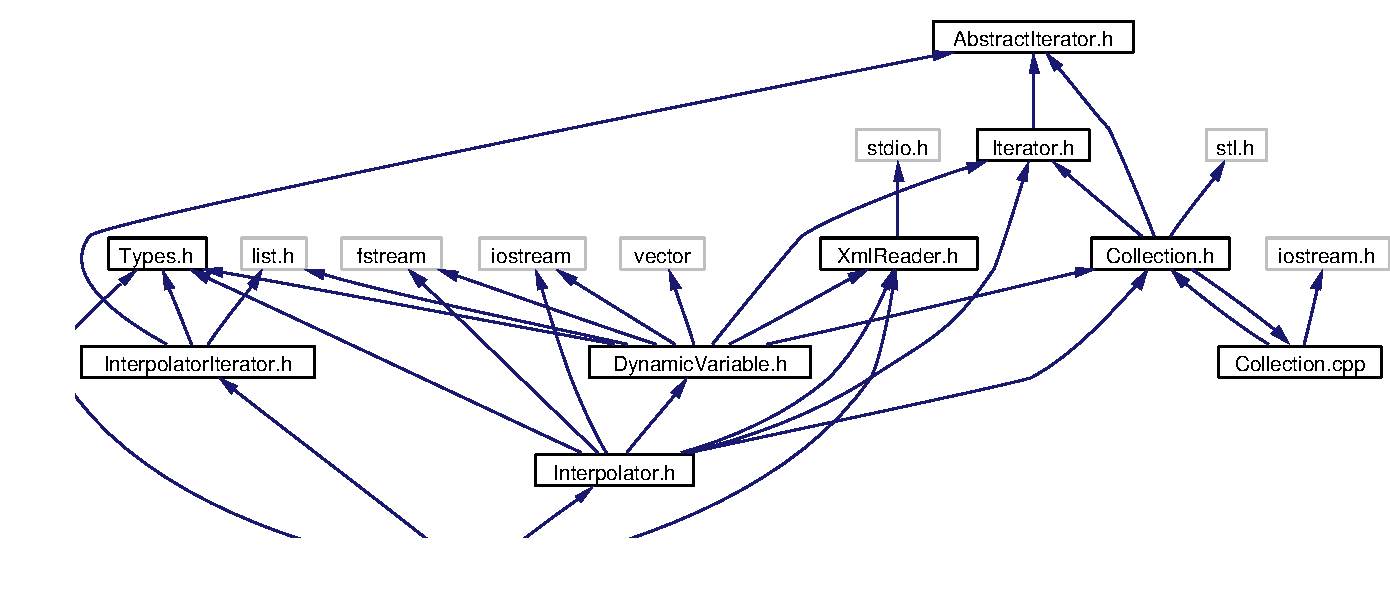
\includegraphics[width=351pt]{InterpolatorTypes_8h__incl}
\end{center}
\end{figure}


This graph shows which files directly or indirectly include this file:\begin{figure}[H]
\begin{center}
\leavevmode
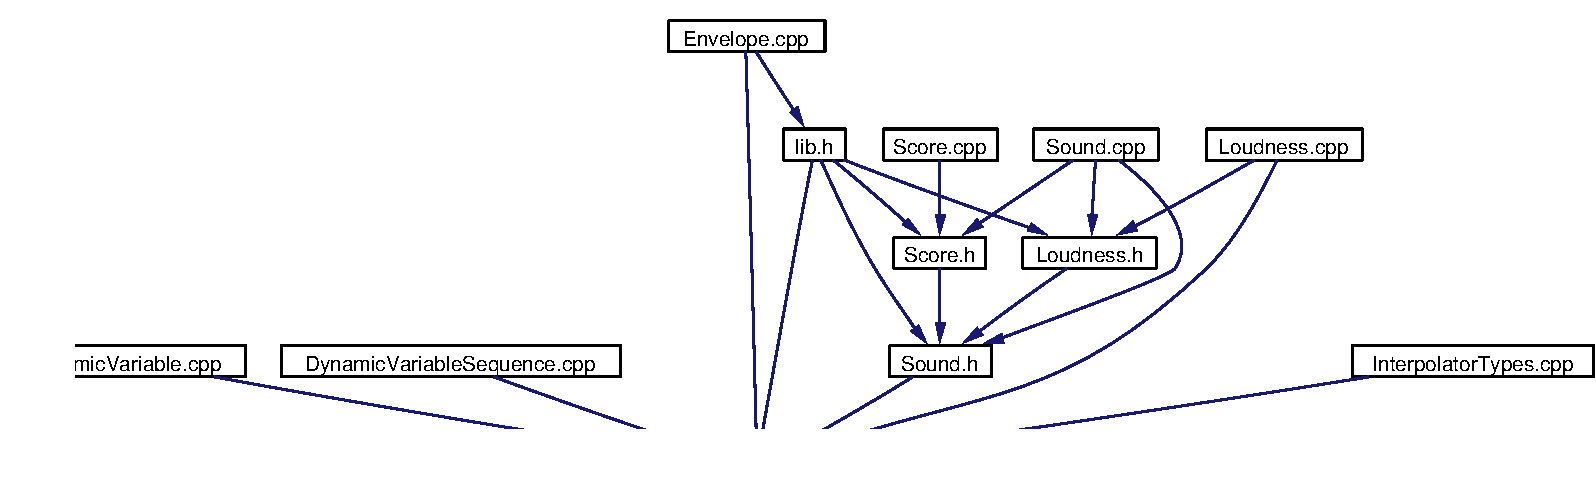
\includegraphics[width=400pt]{InterpolatorTypes_8h__dep__incl}
\end{center}
\end{figure}
\subsection*{Classes}
\begin{CompactItemize}
\item 
class \hyperlink{classCubicSplineInterpolator}{Cubic\-Spline\-Interpolator}
\item 
class \hyperlink{classExponentialInterpolator}{Exponential\-Interpolator}
\item 
class \hyperlink{classLinearInterpolator}{Linear\-Interpolator}
\end{CompactItemize}
